\documentclass{article}[12pt]
\usepackage{enumerate}
\usepackage{amsmath}
\usepackage{tikz}
\usepackage{pgf}
\usepackage{qtree}
\usepackage[localise]{xepersian}

\def\checkmark{\tikz\fill[scale=0.4](0,.35) -- (.25,0) -- (1,.7) -- (.25,.15) -- cycle;} 

\usetikzlibrary{automata, positioning}
\usetikzlibrary{arrows}
\setdigitfont[Scale=1]{PGaramond}
\setlatintextfont[Scale=1]{XB Niloofar}
\settextfont{XB Tabriz}

\شروع{نوشتار}
\شروع{وسط‌چین}
به نام خدا \\

تمرین سری اول
\پایان{وسط‌چین}

\شروع{شمارش}
\فقره \mbox


\begin{LTR}
$S \to \{ S \} | \lambda$ \\
$S \to [ S ] $ \\
$S \to ( S ) $ \\
$S \to SS $
\end{LTR}

\فقره \mbox

\begin{enumerate}
\item \mbox{}
زبان منظم است. چون عبارت منظم زیر برای آن وجود دارد.
\begin{LTR}
$((00+\lambda)^*+(1+111)^*)^*$
\end{LTR}
\item \mbox{}
زبان منظم است. چون عبارت منظم زیر برای آن وجود دارد.
\begin{LTR}
$(((0+1).(0+1).(0+1))^*)+\lambda$
\end{LTR}
\item \mbox{}
\begin{LTR}

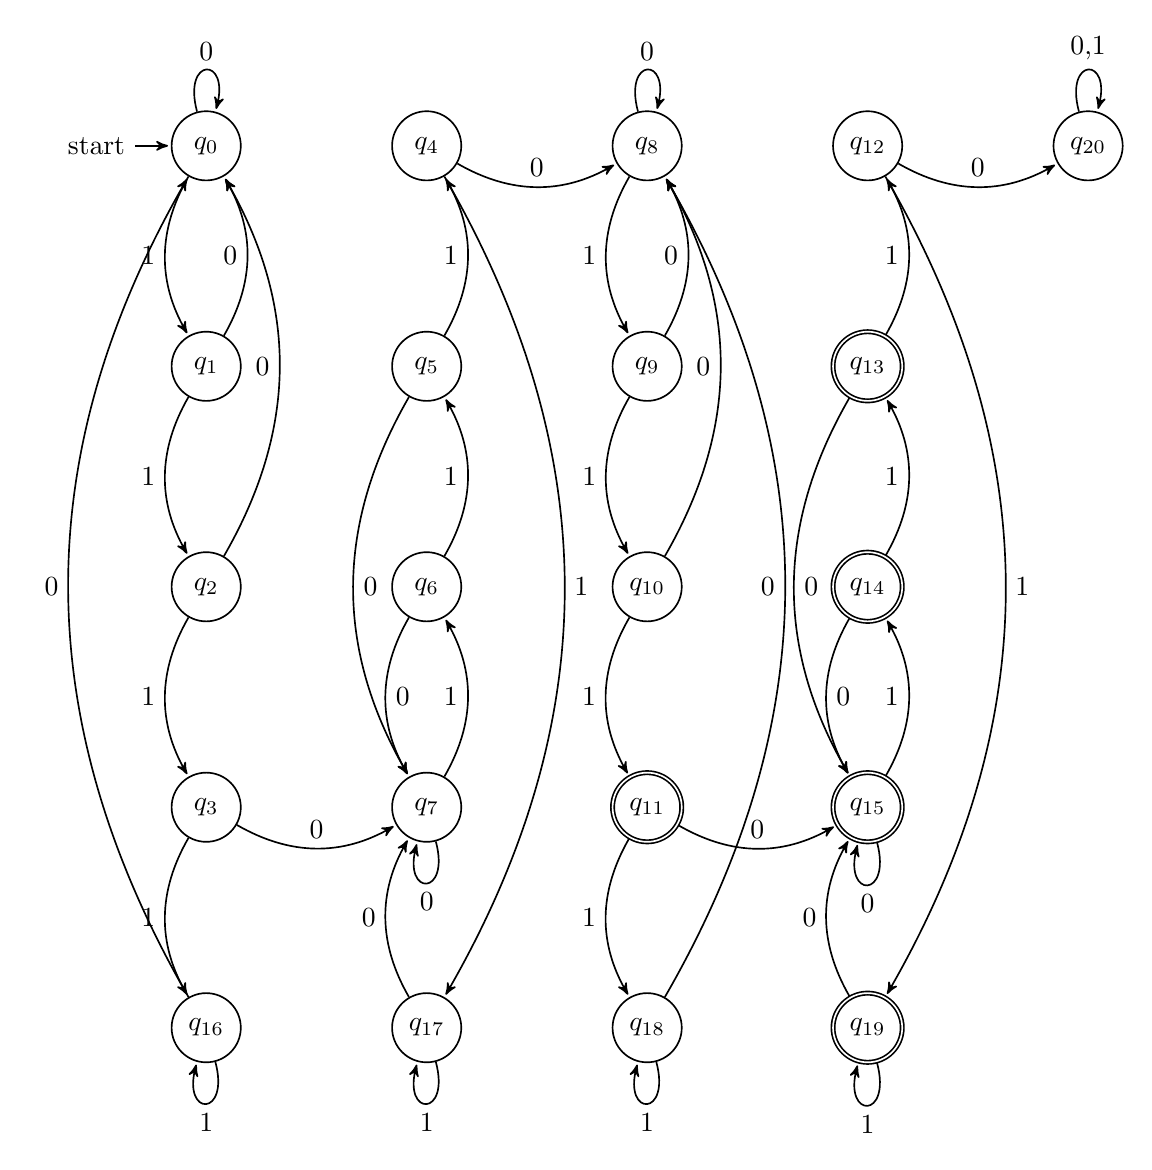
\begin{tikzpicture}[->,>=stealth',shorten >=1pt,auto,node distance=2.8cm,
                    semithick] 
   \node[state,initial] (q_0)   {$q_0$}; 
   \node[state] (q_1) [below of=q_0] {$q_1$}; 
   \node[state] (q_2) [below of=q_1] {$q_2$}; 
   \node[state](q_3) [below of=q_2] {$q_3$};
   \node[state](q_4) [right of=q_0] {$q_4$};
   \node[state](q_5) [below of=q_4] {$q_5$};
   \node[state](q_6) [below of=q_5] {$q_6$};
   \node[state](q_7) [below of=q_6] {$q_7$};
   \node[state](q_8) [right of=q_4] {$q_8$};
   \node[state](q_9) [below of=q_8] {$q_9$};
   \node[state](q_10) [below of=q_9] {$q_{10}$};
   \node[state,accepting](q_11) [below of=q_10] {$q_{11}$};
   \node[state](q_12) [right of=q_8] {$q_{12}$};
   \node[state,accepting](q_13) [below of=q_12] {$q_{13}$};
   \node[state,accepting](q_14) [below of=q_13] {$q_{14}$};
   \node[state,accepting](q_15) [below of=q_14] {$q_{15}$};
   \node[state](q_16) [below of=q_3] {$q_{16}$};
   \node[state](q_17) [below of=q_7] {$q_{17}$};
   \node[state](q_18) [below of=q_11] {$q_{18}$};
   \node[state,accepting](q_19) [below of=q_15] {$q_{19}$};
   \node[state](q_20) [right of=q_12] {$q_{20}$};
   \path[->]
   (q_0) edge [loop above] node {0} ()
	 edge [bend right] node [swap] {1} (q_1)
   (q_1) edge [bend right] node {0} (q_0)
	 edge [bend right] node [swap] {1} (q_2)
   (q_2) edge [bend right] node {0} (q_0)
	 edge [bend right] node [swap] {1} (q_3)
   (q_3) edge [bend right] node {0} (q_7)
	 edge [bend right] node [swap] {1} (q_16)
   (q_16) edge [bend left] node {0} (q_0)
	 edge [loop below] node [swap] {1} ()
   (q_7) edge [bend right] node {1} (q_6)
	 edge [loop below] node {0} ()
   (q_6) edge [bend right] node {1} (q_5)
	 edge [bend right] node {0} (q_7)
   (q_5) edge [bend right] node {1} (q_4)
	 edge [bend right] node {0} (q_7)
   (q_4) edge [bend left] node {1} (q_17)
	 edge [bend right] node {0} (q_8)
   (q_17) edge [bend left] node {0} (q_7)
	 edge [loop below] node [swap] {1} ()
   (q_8) edge [loop above] node {0} ()
	 edge [bend right] node [swap] {1} (q_9)
   (q_9) edge [bend right] node {0} (q_8)
	 edge [bend right] node [swap] {1} (q_10)
   (q_10) edge [bend right] node {0} (q_8)
	 edge [bend right] node [swap] {1} (q_11)
   (q_11) edge [bend right] node {0} (q_15)
	 edge [bend right] node [swap] {1} (q_18)
   (q_18) edge [bend right] node {0} (q_8)
	 edge [loop below] node [swap] {1} ()
   (q_15) edge [bend right] node {1} (q_14)
	 edge [loop below] node {0} ()
   (q_14) edge [bend right] node {1} (q_13)
	 edge [bend right] node {0} (q_15)
   (q_13) edge [bend right] node {1} (q_12)
	 edge [bend right] node {0} (q_15)
   (q_12) edge [bend left] node {1} (q_19)
	 edge [bend right] node {0} (q_20)
   (q_19) edge [bend left] node {0} (q_15)
	 edge [loop below] node [swap] {1} ()
   (q_20) edge [loop above] node {0,1} ();
\end{tikzpicture}
\end{LTR}
\item \mbox{}
زبان منظم نیست، چون لم پامپینگ زیر آن را نقض می‌کند.
شکل کلی جملات به صورت 
$ww^R$
می‌باشد. ما با گرفتن $n$ رشته‌ی زیر را تولید می‌کنیم.
$0^n1^n1^n0^n$
چون ما باید یک زیر رشته از این رشته تولید کنیم. قطعا شامل تعدادی ۰ می‌باشد. با تکرار کردن ۰ ها، یعنی قرار دادن توان ۰ ها به عددی بیش از ۱، رشته‌ی ما از حالت تقارن خارج شده و لم پامپینگ نقض می‌شود، پس این زبان منظم نیست.

\item \mbox{}
زبان منظم است، چون حاصل تفاضل دو زبان منظم است.
\begin{LTR}
$(0+1)^*-(0+1)^*.(011).(0+1)^*$
\end{LTR}
\end{enumerate}
\فقره \mbox
ابتدا تبدیل به
\lr{DFA}
می‌کنیم و سپس آن را کمینه می‌کنیم.
\begin{LTR}
\begin{center}
\begin{tabular}{|c|c|c|c|}
\hline
         &0    &1    &$\lambda^*$\\
\hline
$\to q_0$&$q_1$&-    &$q_1      $\\
\hline
$q_1$    &$q_0$&$q_1$&-          \\
\hline
$q_2$    &$q_2$&$q_1$&-          \\
\hline
\end{tabular}
\end{center}
\begin{center}
\begin{tabular}{|c|c|c|}
\hline
         &$0\lambda^*$&$1\lambda^*$\\
\hline
$\to q_0$&$q_1$       &-           \\
\hline
$q_1$    &$q_0, q_1$  &$q_1$       \\
\hline
$q_0,q_1$&$q_0, q_1$  &$q_1$       \\
\hline
\end{tabular}
\end{center}
\end{LTR}
که همانطور که مشاهده می‌کنید، ما چهار حالت جدید داریم که عبارت است از 
\lr{q0}
و
\lr{q1}
و
\lr{\{q1,q2\}}
هست و همچنین شامل یک حالت 
\lr{trap}
است که در آن تمامی خط تیره‌های موجود در جدول به آن ختم می‌شود\\
\begin{LTR}
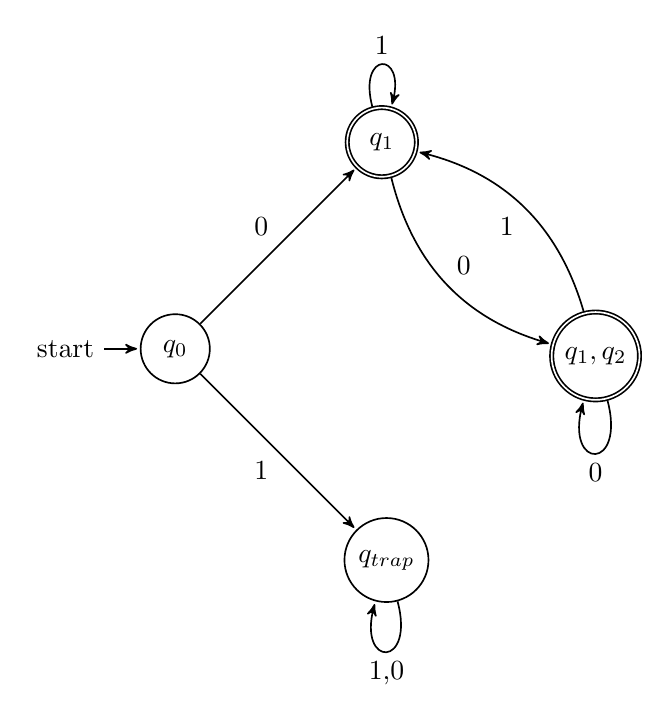
\begin{tikzpicture}[->,>=stealth',shorten >=1pt,auto,node distance=2.8cm,
                    semithick] 
   \node[state,initial] (q_0)   {$q_0$}; 
   \node[state,accepting] (q_1) [above right=of q_0] {$q_1$}; 
   \node[state] (q_3) [below right=of q_0] {$q_{trap}$}; 
   \node[state,accepting](q_2) [below right=of q_1] {$q_1,q_2$};
    \path[->] 
    (q_0) edge  node {0} (q_1)
          edge  node [swap] {1} (q_3)
    (q_1) edge [bend right]  node   {0} (q_2)
          edge [loop above] node {1} ()
    (q_2) edge [bend right] node  {1} (q_1) 
          edge [loop below] node {0} ()
    (q_3) edge [loop below] node  {1,0} ();
\end{tikzpicture}
\end{LTR}

همان طور که مشاهده می‌کنید، حالت‌های $q_1, \{q_1, q_2\}$ با هم معادلند.


\فقره \mbox

اثبات را با استفاده از برهان خلف انجام می‌دهیم.
فرض کنید با کمتر از $2^n$ حالت بتوان رشته‌ها تمام رشته‌های این زبان را تولید کرد. از آنجا که این زبان $2^n$ رشته‌ی پایانی دارد، پس طبق اصل لانه کبوتری می‌توان دو رشته از این زبان را در نظر گرفت که باهم متفاوت هستند ولی حالت پایانی یکسانی دارند. فرض کنید اولین محلی که این دو رشته با هم تفاوت دارند در حرف 
$i$
ام باشد، یعنی 
$w_1=w_i*a$
و 
$w_2=w_i*b$
.چون این دو رشته تا قبل از این با هم هیچ تفاوتی نداشته اند پس هر دوی آن‌ها پس از پارس کردن 
$w_i$
در یک حالت هستند.
اکنون دو رشته‌ی جدید تعریف می‌کنیم به صورت زیر\\
$x=w_1*a^k$
و
$w=w_2*a^k$
\\
حال با اجرای $a^k$ از $w_1$ به یک حالت می‌رسیم $S$ و همچنین با اجرای $a^k$ از $w_2$ نیز به همان حالت می‌رسیم. چون $x$ در زبان هست و $w$ در زبان نیست پس این حالت هم باید پدیرنده باشد و هم رد کننده پس فرض خلف باطل است.
\فقره \mbox 

\شروع{شمارش}

\فقره \mbox

تمامی رشته‌هایی که تعداد برابری \lr{a} و \lr{b} دارند را تولید خواهد کرد.

\فقره \mbox

برای رشته \lr{abab} دو درخت \lr{parse} بصورت زیر وجود دارد.\\

\begin{LTR}

\Tree [.S a [.S b [.S $\lambda$ ] a [.S $\lambda$ ] ] b [.S $\lambda$ ] ]
\Tree [.S a [.S $\lambda$ ] b [.S a [.S $\lambda$ ] b  [.S $\lambda$ ] ] ]

\end{LTR}
\فقره \mbox

گرامر زیر رفع ابهام برای گرامر فوق است:\\
$S\to aBS | bAS | \epsilon$\\
$A\to a | bAA | \epsilon$\\
$A\to b | aBB | \epsilon$


\پایان{شمارش}

\فقره \mbox

\begin{LTR}
\begin{center}
\begin{tabular}{|c c c c c c|}
\hline
     &$q_0$            &$q_1$                 &$q_2$            &$q_3$     &$q_4$\\
$q_1$&$q_1 = q_0$      &                      &                 &          &     \\
$q_2$&$q_3 = q_4$      &$q_1 = q_0, q_3 = q_4$&                 &          &     \\
$q_3$&-                &-                     &-                &          &     \\
$q_4$&$q_1 = q_3$      &$q_3 = q_0$           &$q_3 = q_1 = q_4$&-         &     \\
$q_5$&-                &-                     &-                &\checkmark&-    \\
\hline
\end{tabular}
\end{center}

\begin{center}
\begin{tabular}{|c c c c c c|}
\hline
     &$q_0$            &$q_1$                 &$q_2$            &$q_3$     &$q_4$\\
$q_1$&$q_1 = q_0$      &                      &                 &          &     \\
$q_2$&-                &-                     &                 &          &     \\
$q_3$&-                &-                     &-                &          &     \\
$q_4$&-                &-                     &-                &-         &     \\
$q_5$&-                &-                     &-                &\checkmark&-    \\
\hline
\end{tabular}
\end{center}
\begin{center}
\begin{tabular}{|c c c c c c|}
\hline
     &$q_0$            &$q_1$                 &$q_2$            &$q_3$     &$q_4$\\
$q_1$&\checkmark       &                      &                 &          &     \\
$q_2$&-                &-                     &                 &          &     \\
$q_3$&-                &-                     &-                &          &     \\
$q_4$&-                &-                     &-                &-         &     \\
$q_5$&-                &-                     &-                &\checkmark&-    \\
\hline
\end{tabular}
\end{center}
\end{LTR}
همانطور که مشاهده می‌کنید حالت‌های
\lr{q0, q1} 
و حالت‌های
\lr{q5, q3} 
با هم معادلند.

\فقره \mbox

\begin{enumerate}
\item $A\to aaAb|\epsilon$\\
بله منظم است چون توسط
$(aab)^*$
تولید می‌شود.
\item $A\to AAabb|abb$\\
بله منظم است چون توسط
$(abbabb)^*abb$
تولید می‌شود.
\item $A\to AAabb|\epsilon$\\
بله منظم است چون توسط
$(abbabb)^*abb + \lambda$
تولید می‌شود.
\item $C,D$\\
چون زبان محدود است پس منظم است (کلا شامل ۴ کلمه می‌باشد.)
\item $A\to aA|b$\\
بله منظم است چون توسط
$a(a)^*b$
تولید می‌شود.

\item $A\to (A)|\epsilon$\\
خیر منظم نیست، چون توسط لم پامپینگ زیر پامپ نمی‌شود.

\end{enumerate}

\پایان{شمارش}

\پایان{نوشتار}
